% !TeX root = ../BA_main_englisch.tex
% !TeX spellcheck = en_GB
Machine learning is a subfield of artificial intelligence, `concerned with the question of how to construct computer programs that automatically improve with experience' \cite{Mitchell97}.
Supervised machine learning is one of the three machine learning disciplines, besides unsupervised and reinforcement learning.
The goal is to find a mapping between an input and an output, in our case a drive and its respective optimal transducer policy.
Multiple algorithms to find such a mapping exist, however for high dimensional problems artificial neural networks (ANNs) are often used.
In general, ANNs are a collection of neurons, usually grouped in layers, which are connected and can transmit signals to each other.
The ANN can learn by changing how information is passed through the network.
In the following sections we review two ANN architectures, the fully-connected feedforward ANN and the Long Short-Term Memory (LSTM) network.

\subsection{Fully-connected feedforward ANN}
In this section we review ANNs, following the exposition given in \cite{lu2020dying}.
Let $\textfrak{N}$ be a fully-connected feedforward ANN, meaning there are no loops in the neuron connections and all neurons in a layer are connected to every neuron of the next layer, $\textfrak{N}: \mathbb{R}^{n_1} \to \mathbb{R}^{n_L}$. $n_1$ and $n_L$ denote the dimensionality of the input and output respectively. 
$\textfrak{N}$ has $L$ layers, or columns of neurons.
The network architecture is given by the amount of neurons $n_l$ in each hidden layer $l \in [2, L - 1]$ (see Figure \ref{nn}).
The neurons in layer $l$ are represented by their activations $\vec{a}_l \in \mathbb{R}^{n_l}$, which represent the matrix multiplication output. Additionally each layer includes trainable parameters $W_l \in \mathbb{R}^{n_{l+1} \times n_{l}}$ and $\vec{b}_l \in \mathbb{R}^{n_{l+1}}$ called weights and biases respectively.
The activations can then be calculated using the following formulae \cite{TN_libero_mab2)53517}:
\begin{align*}
	\vec{a}_2 & = W_1 \vec{a}_1 + \vec{b}_1, \\
	\vec{a}_l & = W_{l-1} \xi(\vec{a}_{l-1}) + \vec{b}_{l-1}, \ l \in [3, L],
\end{align*}
where $\xi(x)$ is a function called the activation function applied elementwise. Historically, functions such as $\tanh$ and sigmoid have been used. However, it has been shown in Refs.~\cite{Maas2013RectifierNI, krizhevsky} that the rectified linear unit $\mathrm{ReLU}(x) = \mathrm{max}(0, x)$ often provides better results in fully-connected feedforward ANNs and is used here.

\begin{figure}[h]
	\centering
	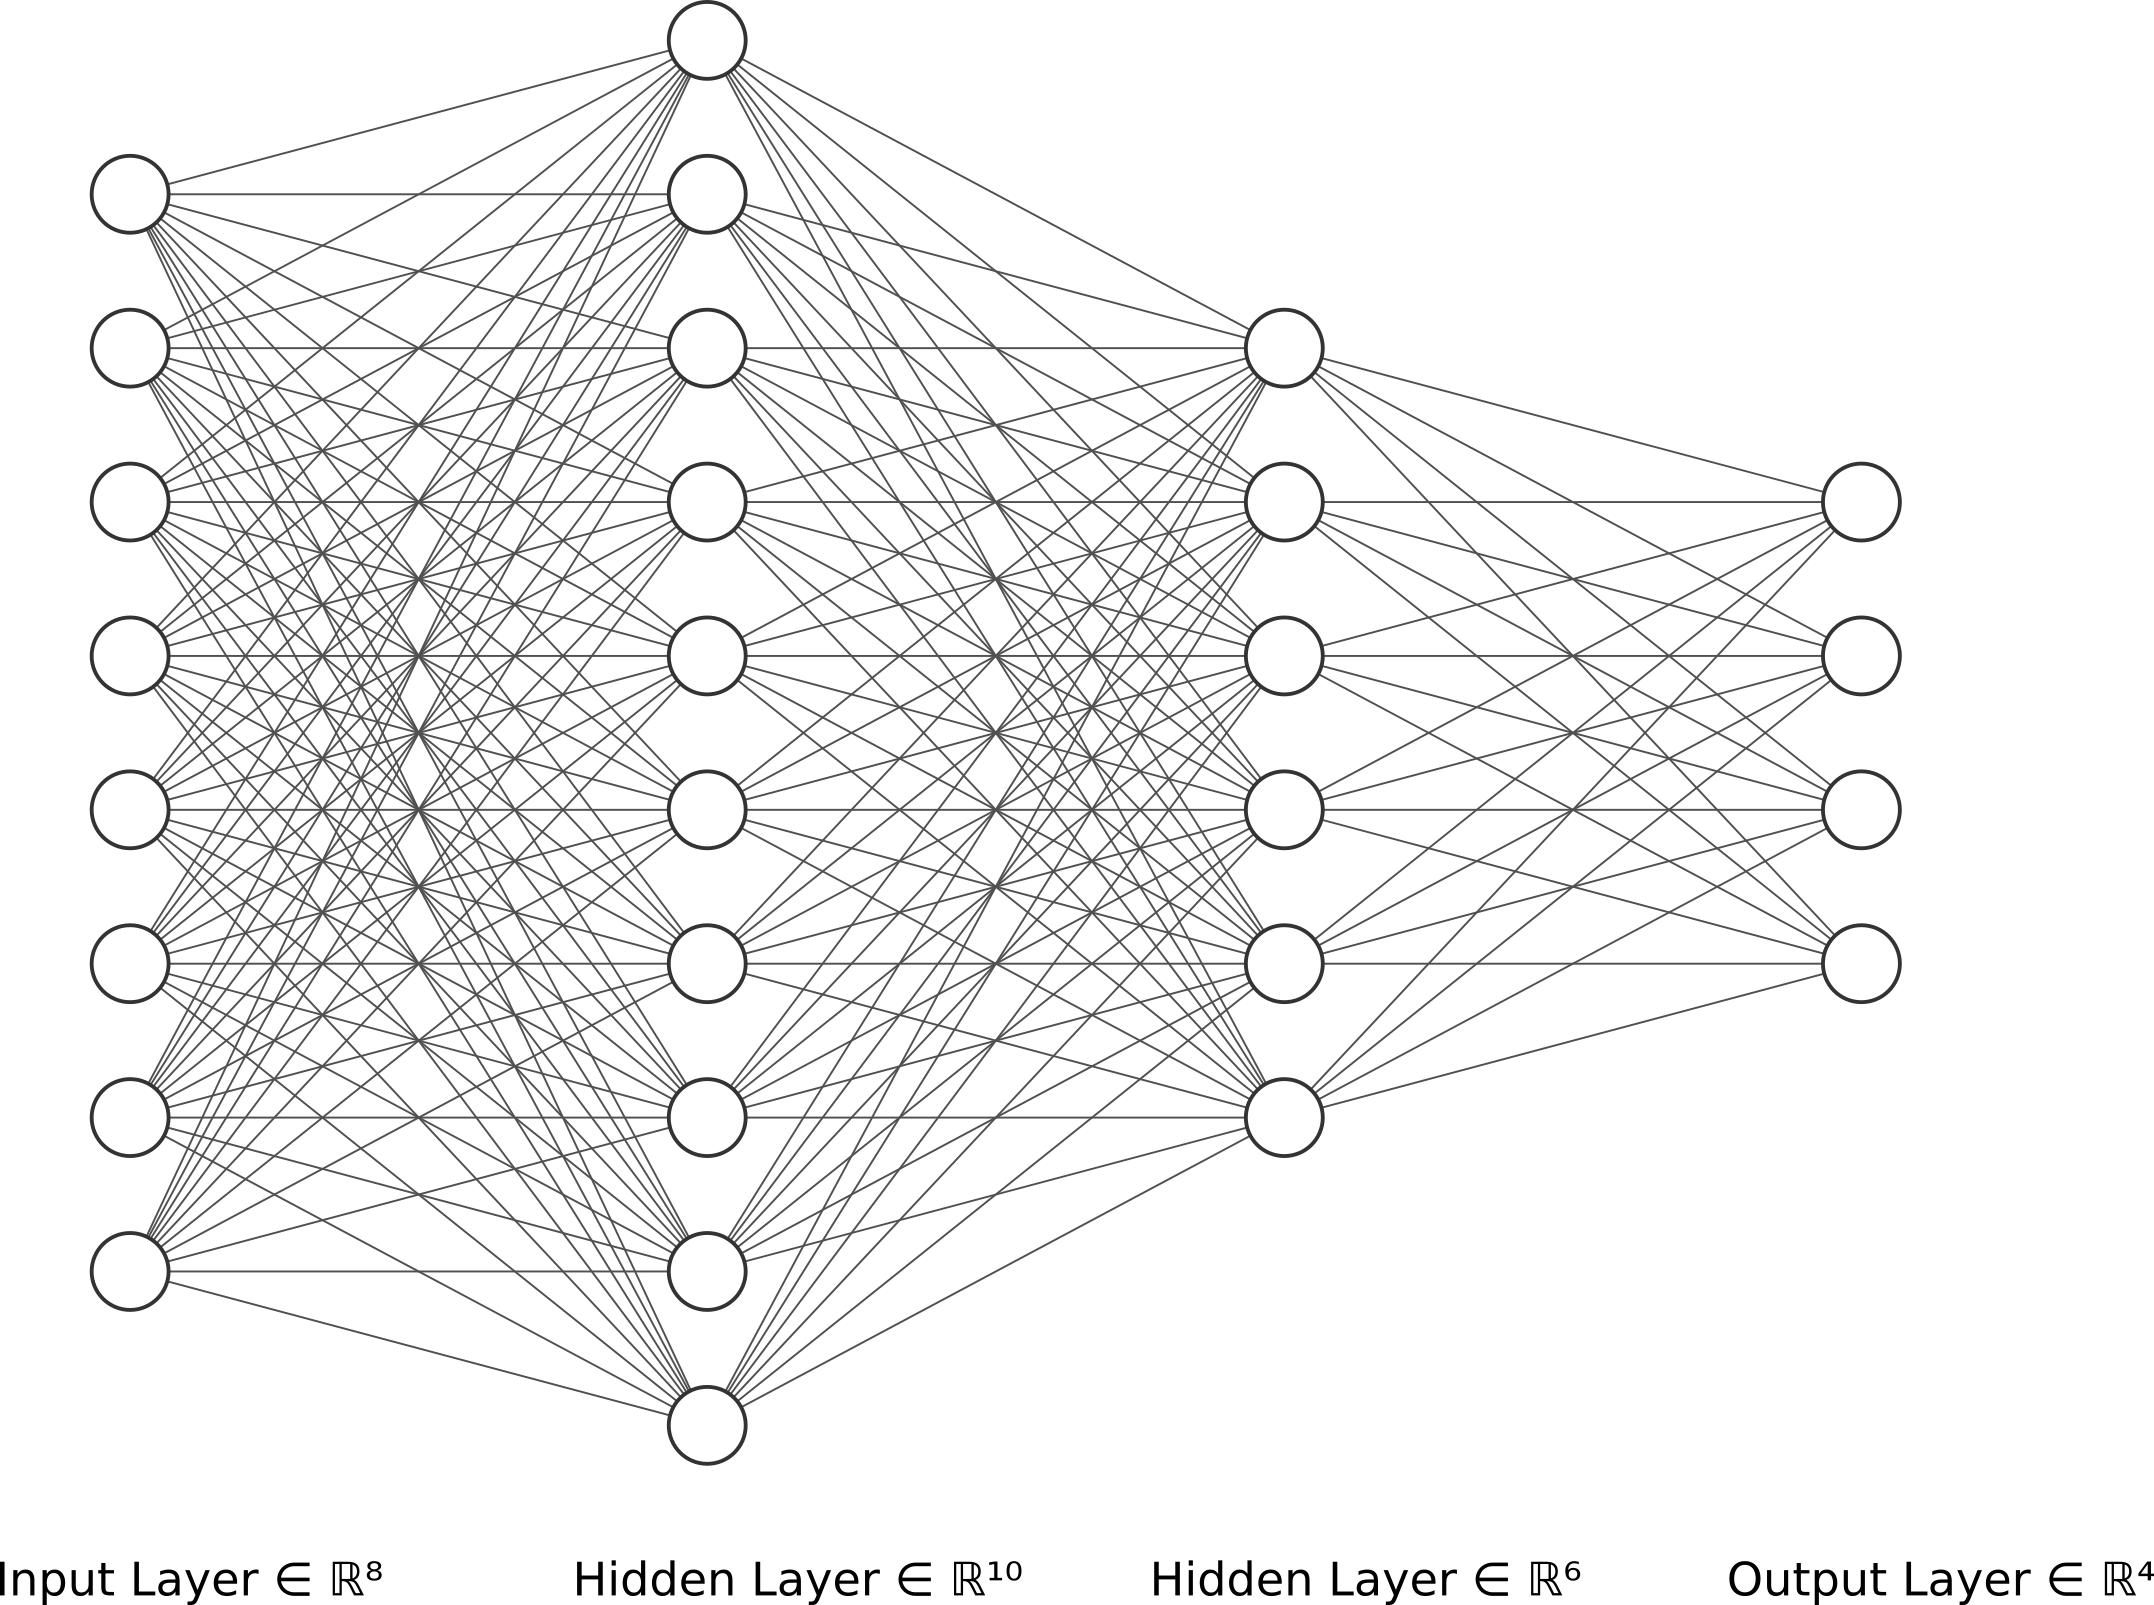
\includegraphics[width=0.75\textwidth]{img/nn}
	\caption{Example of a fully-connected feedforward ANN with four layers, including input, output and two hidden layers \cite{LeNail2019}.}
	\label{nn}
\end{figure}

\subsection{Long Short-Term Memory}
While the network architecture introduced in the previous section performs reasonably well on many problems, it destroys spatial and temporal correlations present in the data. 
So-called convolutional and recurrent networks are often used for these purposes instead, e.g. in image recognition and time series forecasting \cite{10.1007/978-3-642-46466-9_18, 8614252}.

Here we use the LSTM architecture, a type of recurrent neural network (RNN) introduced in \cite{doi:10.1162/neco.1997.9.8.1735}. 
The core idea of RNNs is the usage of loops to store and propagate information through time (Figure \ref{rnn}).
This is fundamentally different to feedforward networks, where information can only travel in one direction.

\begin{figure}[ht]
	\centering
	\includegraphics[width=0.75\textwidth]{img/rnn}
	\caption{Example of a two-layer RNN with LSTM architecture. Each row of LSTM blocks has the same parameters and information is fed into the network sequentially.}
	\label{rnn}
\end{figure}

The network is made up of one or multiple rows of LSTM cells, each of which share parameters.
Figure \ref{lstm} illustrates the internal workings of a single LSTM cell.
Besides the current input $x_t$ and the previous output $h_{t-1}$, the LSTM cell has access to the so-called cell state $c_{t-1}$, which acts as the memory and to which the cell can add and delete information, to compute the output $h_t$.
Internally, the cell is comprised of multiple gates which control the storage of information $i_t, f_t, g_t, o_t$; which are the input, forget, cell and output gates respectively.
The output and gates of each cell are computed using the following equations \cite{NEURIPS2019_9015}:
\begin{align*}
i_t & = \sigma (W_{ii} x_t + b_{ii} + W_{hi} h_{t-1} + b_{hi}), \\
f_t & = \sigma (W_{if} x_t + b_{if} + W_{hf} h_{t-1} + b_{hf}), \\
g_t & = \tanh (W_{ig} x_t + b_{ig} + W_{hg} h_{t-1} + b_{hg}), \\ 
o_t & = \sigma (W_{io} x_t + b_{io} + W_{ho} h_{t-1} + b_{ho}), \\
c_t & = f_t \odot c_{t-1} + i_t \odot g_t, \\
h_t & = o_t \odot \tanh (c_t),
\end{align*}
where $\odot$ and $\sigma(x)$ are elementwise multiplication and application of the sigmoid function respectively.
The input and forget gates $i_t, f_t$ express to what extent new data should be incorporated or deleted from the current cell state $c_t$ respectively.
In contrast to feedforward ANNs, tanh and sigmoid are necessary for the LSTM cell to compute the gate operations.

In some time-series problems, data from a future time step might be required for the current prediction.
In these cases, bidirectional RNNs can provide a better performance.
First introduced in \cite{bidirrnn}, the network is split into a forward and backward part, where the input data is injected in normal and reversed order, respectively.

\begin{figure}[h]
	\centering
	\includegraphics[width=0.75\textwidth]{img/lstm}
	\caption{Visualisation of a single LSTM cell. The input $x_t$ enters the cell in the bottom left and is concatenated with the output $h_{t\text{-}1}$ of the previous cell. The combined data then enters multiple single-layer neural networks represented by orange rectangles with their respective activation functions. The forget gate $f_t$ removes data from the previous cell state $c_{t\text{-}1}$ while $i_t$ and $g_t$ control how new data is added to the memory. $\tanh$ is applied elementwise over the cell state (yellow ellipse) to determine the cell output $h_t$ together with the output gate $o_t$.}
	\label{lstm}
\end{figure}

\newpage

\subsection{Training \& Backpropagation} \label{trainbackprop}
Whereas in the previous sections we considered how information travels through the networks, the question of how one can improve their performance remains.
A \textit{loss} or \textit{cost function} is needed to quantify the dissimilarity between the network predictions and correct values.
It is important that the function is differentiable, as this allows to calculate the gradient of the cost function with respect to the trainable parameters.
The calculation is implemented by the so-called \textit{backpropagation} algorithm \cite{rumelhart1986learning, nielsenneural}, which, in simple terms, uses the chain rule to calculate the gradient.
An \textit{optimiser} such as Adam \cite{kingma2017adam} or Stochastic Gradient Descent (SGD) uses the gradient to update the trainable parameters and move the predictions closer to the desired values.
For \textit{regression} problems such as ours, where one tries to predict a continuous function, the mean squared error (MSE)
\begin{align*}
\mathrm{MSE} = \frac{1}{N} \sum_{i=1}^N (\vec{a}_{L, i} - \vec{y}_i)^2,
\end{align*}
is often used.
The summation is performed over the training data $\{(\vec{x}_i, \vec{y}_i)\}$ with $N$ samples.
$\{\vec{x}_i\}$ is the input, $\{\vec{y}_i\}$ the output data and $\vec{a}_{L, i} = \textfrak{N}(\vec{x}_i)$ the output of the neural network.

Besides the trainable parameters, every machine learning model has one or multiple hyper-parameters.
These values are not changed in training and have to be chosen ahead of time.
An example is the amount of hidden layers and neurons per layer in a fully-connected feedforward ANN.
